\chapter{Measurements}
In the previous sections, we have covered how the quantum system of a qubit coupled to a resonator behaves. In this chapter, we will dive into the readout of the resonator and how it behaves while we are measuring.

\section{I-Q Plane}
\newthought{Based on Hastrup's phd thesis and Knight introduction to quantum optics.}
To understand how a qubit is measured, we must first understand how to the state of the resonator coupled to it. As mentioned earlier, in the dispersive limit, the frequency of the resonator is shifted depending on the qubit. When driven in the proper way, this gives rise to two different kinds of behaviour. How these two are different will be the topic of this chapter. \\

As a start, lets consider the quantum harmonic oscillator subject to $H = \omega^2  x^2 + p^2$ with proper definitions of $x$ and $p$ which properly satisfyes $\comm{x}{p} = i$. To properly diagonalize the Harmonic Oscillator, one usually introduces the raising and lowering operator by:
\begin{align}
    &a \propto x + ip \hfill &a^\dagger \propto x - ip \\
    &x \propto a + a^\dagger \hfill &p\propto i (a - a^\dagger)
\end{align}
Now, one can consider the harmonic oscillator either discretely in the $n = a^\dagger a$ eigenspace or in the continuous basis of $x$ and $p$. The same can be done with photons in a resonator. Where we consider the "quadratures" of the electric field, which we define as Q and I and are defined by the photon creation and annihilation operator in a way quite like the $x$ and $p$ operators of the harmonic oscillator:
\begin{equation}
    Q = a + a^\dagger \hspace{2 cm} I = i(a^\dagger - a)
\end{equation}

\subsection{Coherent States}
\newthought{This is based on Knight} \\ \noindent
When considering a Harmonic Oscillator, the number states have expectation values $\expval{x} = \expval{p} = 0$. To get non-zero values of these expectation values, one is required to have superposition states with adjacent components. Example: $c_n\ket{n} + c_{n+1} \ket{n+1}$, which would satisfy $\expval{x} \propto \expval{a + a^\dagger} \neq 0$. The more natural states would be eigenstates to the annihilation operator:
\begin{equation}
    a \ket{\alpha} = \alpha \ket{\alpha}
\end{equation}
Expanding $\ket{\alpha}$ in the Fock states gives us:
\begin{align}
    a \sum_n C_n \ket{n} = \alpha \sum_{n = 0} C_n \ket{n} \\
    \sum_{n = 1} C_n \sqrt{n} \ket{n - 1}
\end{align}
From where, we can compare the coefficients of the $\ket{n}$:
\begin{equation}
    \sqrt{n} C_n = \alpha C_{n - 1}
\end{equation}
Given $C_0$, we can now determine the rest of the series as:
\begin{equation}
    C_N = \frac{\alpha^n}{\sqrt{n!}} C_0 
\end{equation}
Such that $\ket{\alpha}$ can be found as: 
\begin{equation}
    \ket{\alpha} = C_0 \sum_n \frac{\alpha^n} {\sqrt{n!}} (a^\dagger)^n \ket{0} = C_0
\end{equation}
Where $C_0$ can be found from normalization as:
\begin{align}
    1 &= |C_0|^2 \bra{0}\sum_{n, m}\frac{(\alpha^*)^m} {\sqrt{m!}} a^m \frac{\alpha^n} {\sqrt{n!}} (a^\dagger)^n \ket{0} \\
    1 &= |C_0|^2 \sum_n \frac{|\alpha|^{2n} }{n!} = |C_0|^2 e^{|\alpha|^2} \\
    |C_0|^2 &= e^{-|\alpha|^2}
\end{align}
Which is satisfied by: $C_0 = e^{- |\alpha|^2 / 2}$. Thus a coherent state is given as:
\begin{equation}
    \ket{\alpha} = e^{-|\alpha|^2 / 2} \sum_n \frac{\alpha^n}{\sqrt{n!}} \ket{n}
\end{equation}
Where each complex $\alpha$ corresponds to a coherent state.

\subsection{Overcompleteness / Properties of Coherent States}
\textbf{This is probably relevant for the Q function} 

\subsection{Phase Space Representations}
When considering a way of representing a density matrix $\rho$ in phase space, we have the chance to define the properties we want. A natural way of thinking about this would be probability functions, which have certain properties. It would be useful to be able to express expectation values, $\expval{O} = \Tr{\rho O }$ in phase space. If we were to represent an operator in a coherent basis, it would take the form:
\begin{equation}
    O = \int d\alpha^2 O(\alpha, \alpha^*)\ket{\alpha}\bra{\alpha} 
\end{equation}
The expectation value $\expval{O}$ will now take the form: 
\begin{align*}
    \expval{O} &= \Tr{O \rho} \\
               &= \sum_n \bra{n} \int d\alpha^2 O(\alpha, \alpha^*)\ket{\alpha}\bra{\alpha} \rho \ket{n} \\
               &= \int d\alpha^2 O(\alpha, \alpha^*)\bra{\alpha} \rho \ket{\alpha}
\end{align*}
\marginnote[-1 cm]{Here we have used that $\mel{\alpha}{\rho}{n}$ is a scalar and commutes with the other operators while $\sum_n \ket{n}\bra{n} = \identity$.}
Here $\mel{\alpha}{\rho}{\alpha}$ takes the role of a probability distribution in the coherent phase space. To further ensure that the function is properly normalized, we demand the expectation value of the identity to equal 1:
\begin{align*}
    1 = \expval{\identity} &= \int d\alpha^2 \frac{1}{\pi} \mel{\alpha}{\rho}{\alpha}
\end{align*}
Such that we find the Husimi $Q$-function as:
\begin{equation}
    Q(\alpha) =  \frac{1}{\pi} \mel{\alpha}{\rho}{\alpha}
\end{equation}
which will serve as our probability distribution of a density matrix $\rho$ in the coherent phase space.

\textbf{Should we include the Wigner function in this section? }

\subsection{Common States}
Were we to solve the Hamiltonian in either the position or momentum basis, we would find that the ground state solution to be a Gaussian centered around the bottom of the square-potential and for higher states, we would have some multiplication with a Hermite Polynomial of corresponding order. This fact can be seen in figure \ref{fig:Q_func_examples} where the vacuum state is a 2D gaussian centered at the center (\textit{check validity of statement}). \\
Now for the higher Fock states ($n = 3$ is shown), we see a ring, which is centered with an average radius of $n$. A good intuition for this is the energy conservation of the harmonic oscillator. If we were to measure the position $x=0$ of a harmonic oscillator with non-zero energy, it would certainly have a non-zero momentum. Of course in quantum mechanics this is smeared a bit by Heisenberg Uncertainty Principle.\\
The coherent state described in the previous sections behaves like moving the vacuum around. The center of the distribution will be in $\alpha$.  

\begin{marginfigure}[-6 cm]
    \centering
    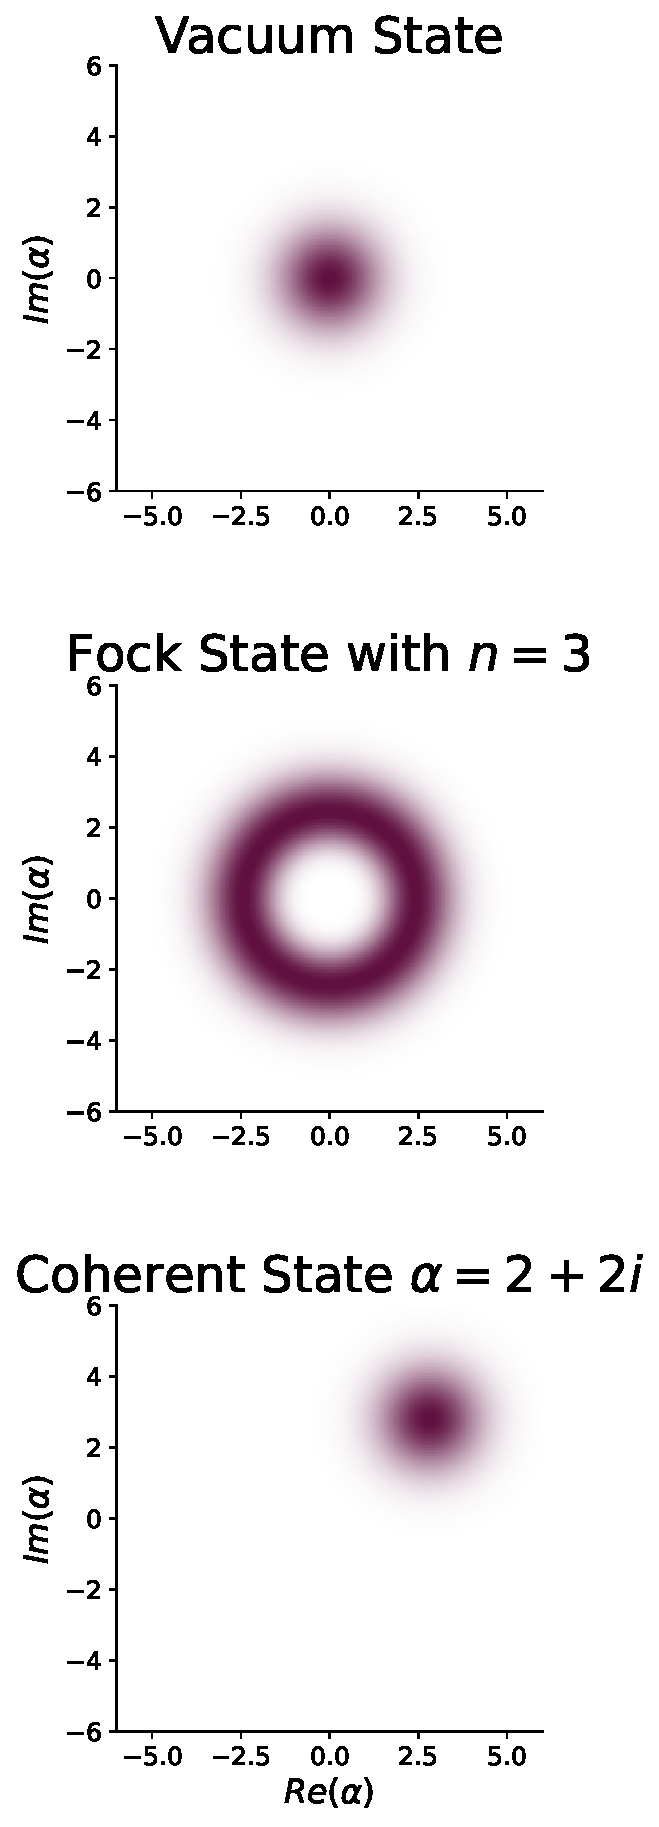
\includegraphics{Figs/Theory/Q_functions.pdf}
    \caption{Example of Different Q-functions for vacuum state, Fock state ($n = 3$) and a coherent state with $\alpha = 2 + 2i$.}
    \label{fig:Q_func_examples}
\end{marginfigure}


\section{Dynamics of a Measured System}
\newthought{The content of this section is based on the excellent review of continuous measurement by Jacobs and Stech \cite{straightforward_introduction}} \\
\noindent
When one first encounter quantum mechanics, the idea of a measurement is an instantaneous and complete projection of a state onto the measured quantity. Measuring an observable given by the hertmitan operator in its eigenbasis, $\mathcal{O} = \sum_n O_n \ket{n}\bra{n}$ (with $\ket{n}$ the eigenstates of O) would thus result in a projection of a state $\ket{\psi}$ onto the state $\ket{n}$ with probability $|\braket{n}{\psi}|^2$ giving a recorded measurement of $O_n$. \marginnote[-1cm]{In the formalism of density matrices the probability is $\mel{n}{\rho}{n}$ and the projected state would be $\ket{n}\bra{n}$. \textbf{Probably switch with text.}} This is considered a strong measurement since it demolishes the state to give an output. When reading out a qubit, we wish to this in a way as to not demolish it, also called Quantum Non-Demolishment readout (QND-readout). For this reason we will introduce the concept of weak measurements and describe how the system behaves while being watched.

\subsection{Positive Operator-Valued Measure (POVM)}
To talk about weak measurements, we first expand the measurement operator to be the set of operators $\Omega_m$, which only condition is that they satisfy the trace preserving condition we used in Section \ref{sec: Quantum Maps}: 
\begin{equation}
    \sum_m \Omega_m^\dagger \Omega_m = \identity 
\end{equation}
Then one can define a measurement with an outcome for each operator:
\begin{equation}
    \rho_f = \frac{\Omega_m\rho\Omega_m^\dagger}{\Tr(\Omega_m \rho \Omega_m^\dagger)}
\end{equation}
where the denominator serves as a renormalization after the outcome $\rho_f$ is observed with the probability $P(m) = \Tr(\Omega_m \rho \Omega_m^\dagger)$. If we now were to check the probability of measuring with the operator between $m = a$ and $m = b$, we would fint:
\begin{equation}
    P(m \in [a, b]) = \sum_{m = a}^b \Tr(\Omega_m\rho\Omega_m^\dagger)
\end{equation}
Or rearranging using linearity and cyclic properties of the trace:
\begin{equation}
    P(m \in [a, b]) = \Tr( \sum_{m = a}^b \Omega_m^\dagger \Omega_m\rho) = \Tr{M \rho}
\end{equation}
where $M = \sum_{m = a}^b \Omega_m^\dagger \Omega_m$ is the positive operator-valued measure (POVM).

\noindent
\textbf{Maybe add the gaussian measurents here to lead up to next section. Integrate section better, what is used? Maybe drop the POVM part and simply call it weak measurements.}

\subsection{Continuous Weak Measurement}
We will consider a weak measurement of a continuous variable, $x$, taking the form of a Gaussian over a time-interval which we divide into pieces of $\Delta t$. At small enough time-steps the strength of the measurement is assumed to be linear with respect to the time such that the operator for measuring associated with $\alpha$ in one time step is (analogue to $m$) \marginnote{\textbf{The "double" normalization constant assures, that if we integrate over whole x and alpha we would have $\identity$}}:
\begin{equation}
    \Omega(\alpha) = \left(\frac{4 k \Delta t}{\pi}\right)^\frac14 \int dx e^{-2k\Delta t (x - \alpha)^2} \ket{x}\bra{x}
\end{equation}
where $\alpha$ is the continuous label and $k$ a measurement strength. If the state of the system is $\rho$ the probability of measuring the operator $\Omega_\alpha$ is then: $P(\alpha) = \Tr\left(\Omega^\dagger(\alpha) \Omega(\alpha) \rho \right)$ \marginnote{For now assuming $\rho$ can be written as $\rho = |\psi(x)|^2 \ket{x}\bra{x}$}, we find 
\begin{align}
    P(\alpha) = \sqrt{\frac{4 k \Delta t}{\pi}} \int_{-\infty}^{\infty} dx |\psi(x)|^2 e^{-4k\Delta t (x - \alpha)^2}
\end{align}
Use $\expval{\alpha} = \expval{X}$\footnote{$\alpha$ and $x$ is symmetric in the gaussian. So writing $\expval{\alpha}$ and exchanging $\alpha \leftrightarrow x$ we integrate over all of the real numbers. Leaving us with an integral over $x|\psi(x)|^2 = \expval{x}$} with $X = x\ket{x}\bra{x}$ and that $\Delta{t}$ so short that $\psi(x)$ is localized around the expectation value compared to the standard deviation of $\frac{1}{\sqrt{8k\Delta t}}$. We then approximate $|\psi(x)|^2 = \delta(x - \expval{X})$ to find:
\begin{equation}
    P(\alpha) = \sqrt{\frac{4 k \Delta t}{\pi}}  e^{-4k\Delta t (\expval{X} - \alpha)^2}
\end{equation}
If one were to "draw" an $\alpha$ from this Gaussian distribution, we will the mean value $\expval{X}$ plus some random contribution from a gaussian with variance $1 / (8k\Delta t)$. We write this as:
\begin{equation}
    \alpha_s = \expval{X} + \frac{\Delta W}{\Delta t \sqrt{8k}}
\end{equation}
Where $\Delta W$ refers to a random Gaussian variable from a distribution with mean $0$ and variance $\Delta t$. 

\subsection{Stochastic Calculus}
The introduction of a stochastic variable forces us to cover some of the fundamental results from stochastic calculus. Most importantly, we use Ito's rules, which governs how to think about the dynamics in an infinitesimal time interval: $dt$ and $dW$.
\begin{enumerate}
    \item $dt^2 \to 0$ - For small timesteps, we disregards second order behaviour. 
    \item $(dW)^2 = dt$. This comes as $dW$ is normally distributed with standard deviation $\sqrt{dt}$ and mean $0$. 
    \item everything of higher order is neglected, such as $dW^3 = dt dW$.
\end{enumerate}
With the above in mind, we can now start analyzing the transformation from $t \to t + dt$, where we need to keep terms of $dt, dW$ and importantly $dW^2 = dt$.

\subsection{Stochastic Evolution}
When going from $\ket{\psi(t)} \to \ket{\psi(t + dt)}$ it will correspond to applying the operator $\Omega_\alpha$ where $\alpha$ is drawn from the probability distribution $P(\alpha)$ to give the stochastic variable $\alpha_s =\expval{X} + {\Delta W}/{\Delta t \sqrt{8k}}$. For now ignoring the normalization, we will get:
\begin{fullwidth}
\begin{align}
    \ket{\psi(t + dt)}  &\propto \Omega(\alpha_s)\ket{\psi(t)} \\
                        &\propto \exp(-2k (\alpha_s - X)^2 dt ) \ket{\psi(t)} \\
                        &\propto \exp(-2k \left({\expval{X} + \frac{dW}{dt \sqrt{8k}}}  - X\right)^2 dt ) \ket{\psi(t)} \\
                        &\propto \exp(-2k X^2 dt + \sqrt{2k} X dW + 4 k X \expval{X} dt) \ket{\psi(t)}
\end{align}
\end{fullwidth}
As we'll normalize later, we were allowed to throw away scalers like $e^{-2k\expval{X}^2}$ and $e^{-\frac{1}{4}dW^2 / dt^2}$ \textbf{check}. Expanding the exponential according to Ito's rules:
\begin{fullwidth}
\begin{equation}
\ket{\psi(t + dt)} \propto    \left( 1 -2k X^2 dt + \sqrt{2k} X dW + 4 k X \expval{X} dt + k X^2 dW^2) \right)\ket{\psi(t)} 
\end{equation}
and letting $dW^2 \to dt$ we obtain:
\begin{equation}
\ket{\psi(t + dt)} \propto    \left( 1 - \left[k X^2 + 4 k X \expval{X} \right]dt + \sqrt{2k} X dW \right)\ket{\psi(t)}     
\end{equation}
\end{fullwidth}
\textbf{Sketch of the rest:} \\ 
\noindent
Normalize to go from $\ket{\psi(t + dt)} = \ket{\psi(t)} + d\ket{\psi(t)}$ to:
\begin{equation}
d|\psi\rangle=\left\{-k(X-\langle X\rangle)^2 d t+\sqrt{2 k}(X-\langle X\rangle) d W\right\}|\psi(t)\rangle .
\end{equation}
With this we get the measurement record given by the stochastic alphas along the way (multiplied by dt):
\begin{align}
    dr = \expval{X}dt + \frac{dW}{\sqrt{8k}}
\end{align}

Now motivate that:
\begin{align}
    d\rho &= (d\ket{\psi})\bra{\psi} + \ket{\psi}(d\bra{\psi}) \\
          &= -k \comm{X}{\comm{X}{\rho}}dt + \sqrt{2k} \left(X\rho + \rho X - 2 \expval{X}\rho \right) 
\end{align}

\subsection{Stochastic Master Equation}
If one compare with the master equation derived earlier, we arrive here by choosing a mapping given by $M_0 = \identity - (iH - K)dt$ and a set of operators $M_\alpha = \sqrt{dt}L_\alpha$ we arrived at the Lindblad Master Equation. We will now repeat the same though process, but instead with the inspiration from the last subsection introduce start with adding a stochastic process to the mapping with a Krauss Operator of the form:
\begin{align}
    M &= \identity - (iH - b)dt + c dW
\end{align}
Such that we use:
\begin{align}
    \rho &\to M\rho M^\dagger = \rho + d\rho
\end{align}
To find;
% \begin{fullwidth}
\begin{align}
    d\rho &= - i \comm{H}{\rho}dt  + (b\rho + \rho b) dt + (c\rho + \rho c)dW + c \rho c^\dagger dt
\end{align}
Where terms of order over $dWdt$ and $dt^2$ are neglected while $dW^2$ is replaced with $dt$. Enforcing the trace preserving condition of the quantum mapping, we must have $\Tr{\rho + d\rho} = 1$, but $\Tr{\rho} = 1$, so $\Tr{d\rho} = 0$. This must be valid for all stochastic evolutions, so we set $dW = 0$ to get the condition: 
\begin{align}
    0 = \Tr(d\rho) = \Tr\left(2 b\rho  + c^\dagger c \rho\right)
\end{align}
Such that $b$ takes the value $b = -\frac{1}{2} c^\dagger c$. And the time evolution takes the form:
\begin{align}
    d\rho &= -i \comm{H}{\rho}dt  -\frac12 (c^\dagger c\rho + \rho c^\dagger c + c \rho c^\dagger) dt \\
    &= -i\comm{H}{\rho}dt + \mathcal{D}[c]\rho dt
\end{align}
Which is simply back at the Lindblad Master equation. If we were to check the same constraint for every $dW$, we would now find:
\begin{equation}
    0 = \Tr(c\rho + \rho c) dW
\end{equation}
But we were at libery to choose a set of Krauss Operators, so we will instead of adding a constraint, simply expand our map to include $M_c = A \sqrt{dW}$:
\begin{equation}
    0 = \Tr(c\rho + \rho c + A \rho A^\dagger) dW
\end{equation}
\textbf{Not entirely good, but we need the term}: $-\expval{c + c^\dagger} \rho$. We should be able to write this in this form. 

We are now back at the equation, we motivated before. And we write the stocastic master equation:
\begin{equation}
    d\rho = -i \comm{H}{\rho}dt + \mathcal{D}[c]\rho dt + \mathcal{H}[c] \rho dW
\end{equation}
Where $\mathcal{H}[c]$ described the stochastic behaviour, which arises from our measurement.

\section{Measuring the state of the Resonator}
\newthought{Use A Quantum Engineers Guide in the beginning.} \\ \noindent
In chapter \ref{sec:qubit-resonator}, we described how the dynamics of the resonator changes depending on the state of the qubit. In this section, we will start with the dispersive equation \ref{eq:two_level_qubit_dispersive}:

\begin{equation}\label{eq:two_level_qubit_dispersive_2}
    H = (\omega_r + \chi \sigma_z) a^\dagger a + \frac12 \omega_{01} \sigma_z
\end{equation}\marginnote[-1cm]{Earlier the frequencies came with tildes, but these have been removed since these are the actual values measured in the labaratory. }

And show how this behaviour translates to what is seen in the phase space of the resonator during a measurement.


\subsection{Homodyne Measurement}


\subsection{Heterodyne Measurement}
